\documentclass[aspectratio=169]{beamer}
\usetheme{default}
\usecolortheme{default}

\usepackage{graphicx}
\usepackage{tikz}
\usepackage{listings}
\usepackage{xcolor}

\setbeamercolor{structure}{fg=black}
\setbeamercolor{frametitle}{bg=white,fg=black}
\setbeamertemplate{navigation symbols}{}
\setbeamertemplate{footline}{}
\setbeamertemplate{headline}{}

\title{AI-Powered Educational Management System}
\subtitle{A Comprehensive Full-Stack Solution with Role-Based Dashboards}
\date{\today}

\begin{document}

% Slide 1: Title Slide
\begin{frame}
\begin{center}
\includegraphics[width=2.5cm]{adypu-logo.png}
\end{center}
\vspace{0.3em}
\begin{center}
{\Large \textbf{AI-Powered Educational Management System}}\\
{\large A Comprehensive Full-Stack Solution with Role-Based Dashboards}
\end{center}
\vspace{0.5em}
\begin{columns}
\begin{column}{0.55\textwidth}
\small
\textbf{Name:} Priyanshu Kumar Sharma \\
\textbf{Program:} BTech IT (CTIS) \\
\textbf{URN No:} 2022-B-17102004A \\
\textbf{Project Id:} Your Project ID \\
\textbf{Team Members:} \\
\quad • Vaishnavi Jadhav \\
\quad • Vaibhav Gulage
\end{column}
\begin{column}{0.45\textwidth}
\small
\raggedleft
\textbf{Guide Name:} \\
Prof. Prini Rastogi
\end{column}
\end{columns}
\end{frame}

% Slide 2: Table of Contents
\begin{frame}{Table of Contents}
\begin{itemize}
\item Introduction
\item Problem Statement
\item Literature Review
\item Research Methodology
\item System Architecture
\item Key Features
\item AI Integration
\item Implementation
\item Demo
\item Deployment
\item Future Scope
\item References
\item Conclusion
\end{itemize}
\end{frame}

% Slide 3: Introduction & Problem Statement
\begin{frame}{Introduction \& Problem Statement}
\textbf{Project Overview:}
\begin{itemize}
\item \textbf{AI-Powered Educational Management System}
\item Full-Stack Web Application with role-based dashboards
\item Target Users: Administrators, Teachers, Students
\item Bilingual support (English/Hindi)
\end{itemize}

\textbf{Problem Statement:}
\begin{itemize}
\item Traditional systems lack digital integration and AI support
\item Limited personalized learning and real-time collaboration
\item Manual processes and language barriers
\item Need for unified platform with intelligent features
\end{itemize}

\textbf{Solution:} Comprehensive AI-powered platform addressing all stakeholder needs
\end{frame}

% Slide 4: Literature Review
\begin{frame}{Literature Review}
\textbf{Existing Systems Analysis:}
\begin{itemize}
\item \textbf{Moodle LMS [1]:} Open-source LMS, limited AI integration
\item \textbf{Google Classroom [2]:} Cloud-based platform, lacks AI tutoring
\item \textbf{Khan Academy [3]:} Personalized dashboards, basic adaptive learning
\item \textbf{Blackboard Learn [4]:} Enterprise LMS, limited multilingual support
\item \textbf{Coursera [5]:} MOOC platform, focuses on higher education
\end{itemize}

\textbf{Key Limitations:}
\begin{itemize}
\item Limited AI integration and personalization
\item Poor real-time collaboration features
\item Inadequate multilingual support
\item Traditional assessment methods
\end{itemize}

\textbf{Research Gap \& Our Contribution:}
\begin{itemize}
\item Comprehensive AI integration across all user roles
\item Real-time bilingual support with live translation
\item Unified platform combining LMS, AI tutoring, and development tools
\end{itemize}
\end{frame}

% Slide 5: Research Methodology
\begin{frame}{Research Methodology}
\begin{columns}
\begin{column}{0.5\textwidth}
\textbf{Development Approach:}
\begin{itemize}
\item Agile Methodology
\item Full-Stack Development
\item API-First Design
\item Component-Based Architecture
\end{itemize}

\textbf{AI Integration Algorithm:}
\begin{itemize}
\item User query preprocessing
\item Intent classification using NLP
\item OpenAI API integration
\item Real-time translation
\item Response optimization
\end{itemize}
\end{column}
\begin{column}{0.5\textwidth}
\begin{center}
\begin{tikzpicture}[scale=0.4]
\node[draw,rounded corners,fill=green!20] (start) at (0,6) {Start};
\node[draw,rectangle,fill=blue!20] (login) at (0,4.5) {User Login};
\node[draw,diamond,fill=yellow!20] (role) at (0,3) {Role Check};
\node[draw,rectangle,fill=red!20] (admin) at (-3,1.5) {Admin};
\node[draw,rectangle,fill=orange!20] (teacher) at (0,1.5) {Teacher};
\node[draw,rectangle,fill=purple!20] (student) at (3,1.5) {Student};
\node[draw,rectangle,fill=cyan!20] (ai) at (0,0) {AI Processing};

\draw[->] (start) -- (login);
\draw[->] (login) -- (role);
\draw[->] (role) -- (admin);
\draw[->] (role) -- (teacher);
\draw[->] (role) -- (student);
\draw[->] (admin) -- (ai);
\draw[->] (teacher) -- (ai);
\draw[->] (student) -- (ai);
\end{tikzpicture}
\end{center}
\end{column}
\end{columns}
\end{frame}

% Slide 6: System Architecture & Features
\begin{frame}{System Architecture \& Features}
\begin{columns}
\begin{column}{0.5\textwidth}
\textbf{Tech Stack:}
\begin{itemize}
\item \textbf{Frontend:} React.js, Tailwind CSS
\item \textbf{Backend:} Node.js, Express.js
\item \textbf{Database:} MongoDB Atlas
\item \textbf{AI APIs:} OpenAI, Google Translate
\item \textbf{Deployment:} Docker, Nginx
\end{itemize}

\textbf{Key Features:}
\begin{itemize}
\item \textbf{Admin:} User management, analytics
\item \textbf{Teacher:} Virtual classroom, quiz management
\item \textbf{Student:} AI tutor, virtual code editor
\item \textbf{Common:} Real-time communication, bilingual support
\end{itemize}
\end{column}
\begin{column}{0.5\textwidth}
\begin{center}
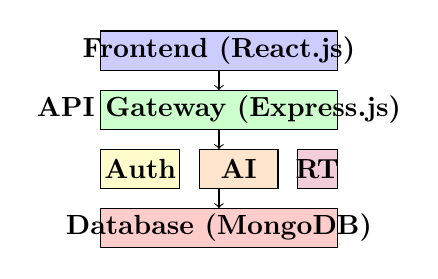
\begin{tikzpicture}[scale=0.5]
\draw[fill=blue!20] (0,4) rectangle (6,5);
\node at (3,4.5) {\textbf{Frontend (React.js)}};

\draw[fill=green!20] (0,2.5) rectangle (6,3.5);
\node at (3,3) {\textbf{API Gateway (Express.js)}};

\draw[fill=yellow!20] (0,1) rectangle (2,2);
\node at (1,1.5) {\textbf{Auth}};

\draw[fill=orange!20] (2.5,1) rectangle (4.5,2);
\node at (3.5,1.5) {\textbf{AI}};

\draw[fill=purple!20] (5,1) rectangle (6,2);
\node at (5.5,1.5) {\textbf{RT}};

\draw[fill=red!20] (0,-0.5) rectangle (6,0.5);
\node at (3,0) {\textbf{Database (MongoDB)}};

\draw[->] (3,4) -- (3,3.5);
\draw[->] (3,2.5) -- (3,2);
\draw[->] (3,1) -- (3,0.5);
\end{tikzpicture}
\end{center}
\end{column}
\end{columns}
\end{frame}

% Slide 7: AI Integration & Implementation
\begin{frame}{AI Integration \& Implementation}
\begin{columns}
\begin{column}{0.5\textwidth}
\textbf{AI Components [6-8]:}
\begin{itemize}
\item \textbf{AI Tutor:} ChatGPT-powered assistance
\item \textbf{Translation:} Real-time language support
\item \textbf{Proctoring:} TensorFlow.js monitoring
\item \textbf{Analytics:} ML-based insights
\end{itemize}

\textbf{Database Schema:}
\begin{itemize}
\item \textbf{User:} username, role, credentials
\item \textbf{Teacher:} qualifications, subjects
\item \textbf{Student:} enrollment, performance
\item \textbf{Classroom:} sessions, materials
\end{itemize}
\end{column}
\begin{column}{0.5\textwidth}
\begin{center}
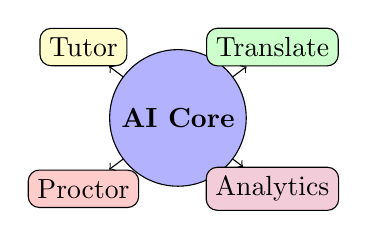
\begin{tikzpicture}[scale=0.6]
\node[draw,circle,fill=blue!30,minimum size=1.5cm] (ai) at (0,0) {\textbf{AI Core}};

\node[draw,rounded corners,fill=yellow!20] (tutor) at (-2,1.5) {Tutor};
\node[draw,rounded corners,fill=green!20] (translate) at (2,1.5) {Translate};
\node[draw,rounded corners,fill=red!20] (proctor) at (-2,-1.5) {Proctor};
\node[draw,rounded corners,fill=purple!20] (analytics) at (2,-1.5) {Analytics};

\draw[->] (ai) -- (tutor);
\draw[->] (ai) -- (translate);
\draw[->] (ai) -- (proctor);
\draw[->] (ai) -- (analytics);
\end{tikzpicture}
\end{center}

\textbf{Authentication:} JWT-based with RBAC [9]
\end{column}
\end{columns}
\end{frame}

% Slide 8: Demo & Deployment
\begin{frame}{Demo \& Deployment}
\begin{columns}
\begin{column}{0.5\textwidth}
\textbf{Demo Credentials:}
\begin{center}
\begin{tabular}{|c|c|}
\hline
\textbf{Role} & \textbf{Login} \\
\hline
Admin & admin/admin123 \\
\hline
Teacher & teacher1/teacher123 \\
\hline
Student & student1/student123 \\
\hline
\end{tabular}
\end{center}

\textbf{Access URLs:}
\begin{itemize}
\item Frontend: \texttt{localhost:3000}
\item Backend: \texttt{localhost:5000}
\end{itemize}
\end{column}
\begin{column}{0.5\textwidth}
\textbf{Deployment [10-11]:}
\begin{itemize}
\item \textbf{Containerization:} Docker Compose
\item \textbf{Web Server:} Nginx reverse proxy
\item \textbf{Environment:} Node.js runtime
\item \textbf{Database:} MongoDB Atlas cloud
\end{itemize}

\textbf{Quick Start:}
\begin{itemize}
\item \texttt{docker-compose up -d}
\item Automated dependency installation
\item Production-ready deployment
\end{itemize}
\end{column}
\end{columns}
\end{frame}

% Slide 9: Future Scope
\begin{frame}{Future Scope}
\textbf{Platform Extensions [12-13]:}
\begin{itemize}
\item \textbf{Mobile Apps:} Native iOS/Android with offline capabilities
\item \textbf{AR/VR Learning:} Immersive virtual classrooms
\item \textbf{Blockchain:} Secure credential verification
\item \textbf{IoT Integration:} Smart classroom devices
\end{itemize}

\textbf{AI Enhancements:}
\begin{itemize}
\item \textbf{Personalized Learning:} AI-driven curriculum customization
\item \textbf{Emotion Recognition:} Student engagement detection
\item \textbf{Advanced Proctoring:} Behavioral analysis
\end{itemize}

\textbf{Real-world Impact:}
\begin{itemize}
\item Digital divide reduction in rural areas
\item Cost-effective education delivery
\item Global accessibility to quality education
\item Contributing to \$350B+ EdTech market [14]
\end{itemize}
\end{frame}

% Slide 10: References
\begin{frame}{References}
\tiny
\begin{enumerate}
\item M. Dougiamas and P. Taylor, "Moodle: Using learning communities to create an open source course management system," \textit{Proc. EDMEDIA}, pp. 171-178, 2003.
\item A. Iftakhar, "Google classroom: what works and how?," \textit{Journal of Education and Social Sciences}, vol. 3, no. 1, pp. 12-18, 2016.
\item S. Khan, "The one world schoolhouse: Education reimagined," \textit{Twelve Books}, 2012.
\item R. Beatty and C. Ulasewicz, "Faculty perspectives on moving from Blackboard to the Moodle learning management system," \textit{TechTrends}, vol. 50, no. 4, pp. 36-45, 2006.
\item D. Koller et al., "Retention and intention in massive open online courses," \textit{Proc. ACM Conference on Learning}, pp. 781-790, 2013.
\item T. Brown et al., "Language models are few-shot learners," \textit{Advances in Neural Information Processing Systems}, vol. 33, pp. 1877-1901, 2020.
\item Y. Wu et al., "Google's neural machine translation system," \textit{arXiv preprint arXiv:1609.08144}, 2016.
\item M. Abadi et al., "TensorFlow: Large-scale machine learning on heterogeneous systems," \textit{Proc. OSDI}, pp. 265-283, 2016.
\item A. Silberschatz et al., "Operating system concepts," \textit{John Wiley \& Sons}, 2018.
\item D. Merkel, "Docker: lightweight linux containers for consistent development and deployment," \textit{Linux Journal}, vol. 2014, no. 239, pp. 2, 2014.
\item F. Reale et al., "Nginx: a practical guide to high performance," \textit{O'Reilly Media}, 2018.
\item S. Nakamoto, "Bitcoin: A peer-to-peer electronic cash system," \textit{Decentralized Business Review}, 2008.
\item P. Milgram and F. Kishino, "A taxonomy of mixed reality visual displays," \textit{IEICE Trans. Information and Systems}, vol. 77, no. 12, pp. 1321-1329, 1994.
\item Global Market Insights, "E-learning Market Size By Technology," \textit{Industry Analysis Report}, 2023.
\item J. Sweller, "Cognitive load theory," \textit{Psychology of Learning and Motivation}, vol. 55, pp. 37-76, 2011.
\end{enumerate}
\end{frame}

% Slide 11: Conclusion
\begin{frame}{Conclusion}
\textbf{Key Achievements:}
\begin{itemize}
\item Comprehensive educational ecosystem with role-based access
\item AI-powered intelligent tutoring and real-time assistance
\item Bilingual support breaking language barriers
\item Modern scalable architecture with Docker deployment
\item Real-time communication and collaboration features
\end{itemize}

\textbf{Technical Contributions:}
\begin{itemize}
\item Integration of multiple AI APIs (OpenAI, Google Translate, TensorFlow.js)
\item Unified platform combining LMS, AI tutoring, and development tools
\item JWT-based authentication with role-based access control
\end{itemize}

\textbf{Impact:} Transforming traditional education through innovative technology solutions that enhance learning experiences for all stakeholders.

\vspace{1em}
\begin{center}
\textbf{Thank You!}\\
\textbf{Questions \& Discussion}
\end{center}
\end{frame}

\end{document}